\chapter{Hardware}
\section{Einführung}
In diesem Kapitel werde ich auf die verwendete Hardware eingehen, die wir für unser Passiv Radar verwendet haben. Die Signalverarbeitung haben wir mit zwei SDR bewerkstelligt, da diese recht erschwinglich sind. SDRs gibt es schon für bis zu 20 Euro jedoch kamen diese für uns nicht frage, da sie für unser Signal eine zu geringe Bandbreite haben. Jedoch benötigen wir eine Bandbreite von mindestens 5 MHz um unser gesamtes Signal aufzeichnen zu können. Nachdem wir uns hier ein wenig umgeschaut haben und verschiedene SDR miteinander verglichen haben wir uns letzthin für zwei ADALM-PLUTO SDRs entschieden. Bei den Antennen verwenden wir zwei DVB-T die sind zwar nicht gut eingestellt und vermessen aber dafür recht billig. Damit unsere beiden SDRs synchron arbeiten brauchten wir noch einen externen Taktgeber hier verwenden wir eine  GPS-stabilisierter Oszillator. Um unsere Antennen präzise ausrichten zu können benutzen wir pro Antenne noch einen Antennenständer. Das komplett fertige Setup ist in Abbildung zu sehen.
\section{Pluto-SDR}


\section{Antenne}
Wir benutzen für unser Passiv-Radar zwei Antennen die für DVB-T gedacht sind. Die Antenne ist ein Yagi Antenne mit 43 Elementen wie man im Abbildung /ref{antenne} sieht die im Frequenzbereich von 470 bis 862 MHZ arbeitet, was für unseren Anwendungsfall sehr gut geeignet ist.
Die Daten zur Antenne stehen in der Tabelle. Antennen Daten:\\ \\
\begin{tabular}[h]{rl}
    Antenne         & SKT SL43-01 UHF 43            \\
    Antennengewinn  & 11..13 dB                     \\
    Frequenzbereich & 470-862 MHz                   \\
    Halbwertsbreite & horiz. 30...40°/ver. 35...50° \\
\end{tabular}

\begin{figure}
    \centering
    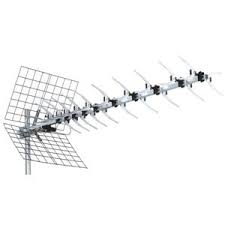
\includegraphics[width=\textwidth]{images/antenne.png}
    \caption{SKT SL43-01 UHF 43  Antenne}\label{antenne}
\end{figure}

\section{Clock}